\label{sec:data}
% Dataset	and	variables
% • Main	characteristics	of	the	dataset:	source,	type	of	data,	…
% • Description	of	variables	used	for	the	analysis	and	correspondence
% with	the	(ideal)	magnitudes	in	the	empirical	specification
% • Descriptive	statistics	of	the	main	variables	in	the	analysis
\subsection{The PITEC panel of Spanish firms}
\label{subsec:pitec}
The final 2016-version of the PITEC panel contains yearly responses till 2016 from firms with at least one employee. 7,283 firms are observed since the first year of the panel survey, 2003. This first wave was constructed by joining two panels of which the first is a panel of 7,264 firms with 200 or more employees, covering 86\% of all firms with 200 or more employees at the time; the other panel contains 3,794 small and medium-sized enterprises (SMEs) according to 56\% of firms with less than 200 employees that carry out internal R\&D activities \citep{vega2009does}. New to the 2004 wave of the survey is the introduction of 3,040 new firms to the panel of which 437 were SMEs with external R\&D expenses only and about 1,000 were SMEs without R\&D expenditure.\footnote{Description of the methodology, the full questionnaires etc. in PITEC is available by the Spanish Foundation of Science \& Technology at \href{https://icono.fecyt.es/pitec}{icono.fecyt.es/pitec}} Additionally 2,480 SMEs with internal R\&D activities are added to the panel in the 2005 wave of the panel.

Thus, the panel is unbalanced and to include the higher number of firms I limit the time span to 2005-2016 providing a balanced panel of 12,803 firms. 46 firms are added in later waves, but these and 705 others are dropped due to missing information in 2005. Due to firms stopping to respond to the survey I need to drop 200-500 firms from the panel each of the following waves, but for 2014 and 2016 where 2,000 and 700 firms are dropped respectively, leaving us with a total of 5,662 firms with full information, 44\% of the original 2005-sample. The data set does not allow us to  convincingly distinguish between firms ceasing to exist, deliberate non-responses, and random non-responses. However, that 60\% of firms still answered the survey in 2016 indicates a sizeable random non-response rate in the previous years. Most of the firms failing to answer the survey in one or more years are smaller firms of which half of them have 30 employees at most, even more so, heterogeneity in the response rate is also present between the different industries, especially outside of the service sector.
\footnote{The range is from 46\% of the firms having missing information for one or more years in both the "chemicals, pharmaceuticals, plastics, ceramics \& petrol" and "foods, beverages \& tobacco" industries to 66\% in construction, 69\% of the firms in "furniture, games, toys, \& other manufacturing" and 91\% within "agriculture and resource extraction".}
Due to low sample sizes and a expectedly much different innovation processes I drop a total of 305 firms mainly engaged in agriculture, resource extraction, recycling, energy, water, sanitation, or construction. There can be fundamental differences in the innovative processes even between the manufacturing and service sector \citep{hoffman1998small} as well as in the outcomes \citep{harrison2014does}, thus, of the remaining 5,357 firms only the subsample of 3,013 manufacturing firms are analyzed, leaving out the 2,344 firms in the service sector.

\subsection{Indicator of innovation success}
\label{subsec:proxies}
The dependent variable is new products the share of new products unique to the firm measured as the share of total revenue. Thus, it is not only an indicator of innovation in products but of the commercial success of product innovations. The variable is worked out as the sale of products introduced within the same financial year as well as products introduced within the two prior years. Therefore different length of leads $k\in0,1,2,3$ is tried out in the regression such that $new_{t+k}$ is determined by the independent variables at period $t$.

\subsection{Determinants of innovation}
\label{subsec:determinants}
The main time-varying determinants used are the percentage of total employees engaged in internal R\%D activities $pidp_t$, a dummy $idin_t$ for having expenses on internal R\&D activities, and a dummy $exter_t$ for only having external R\&D expenditures.

Furthermore, for the Random Effects estimation industry dummies and regional effects dummies for Madrid, Catalonia, and Andalusia are included.

\subsection{Descriptive statistics}
\label{subsec:descriptive}
Table \ref{tab:descriptive} show mean and standard deviation of the key variables sorted by the different industries within manufacturing. Heterogeneity is present throughout including the row showing the correlations $corr(new_{t+2},pidp_t)$.
\begin{table}[H]
  \centering
  \caption{Descriptive statistics}
  \footnotesize
    \begin{tabular}{l*{3}{c}}
\hline\hline
                    &\multicolumn{3}{c}{}                  \\
                    &           0&           1&       Total\\
 &Manufacturing &Services\\\midrule
Sales of new products in year t+1&16.81 (28.54)&13.58 (26.56)&15.70 (27.92)\\
[1em]
log R\&D expenses at region-level&0.698 (0.321)&0.659 (0.349)&0.685 (0.332)\\
[1em]
log internal R\&D expenses&0.925 (0.871)&1.615 (1.594)&1.162 (1.217)\\
[1em]
log external R\&D expenses&0.222 (0.480)&0.376 (0.813)&0.275 (0.620)\\
[1em]
Cont. of basic research&0.426 (0.588)&0.425 (0.606)&0.426 (0.594)\\
[1em]
Cont. of applied research&1.577 (0.903)&1.381 (0.924)&1.509 (0.915)\\
[1em]
Cont. of tehcnological development&1.729 (0.862)&1.674 (0.865)&1.710 (0.864)\\
[1em]
Cont. of external R\&D only&0.154 (0.386)&0.134 (0.355)&0.147 (0.376)\\
\midrule Number of firms&1,949&1,026&2,975\\ Total observations&21,439&11,286&32,725\\
\midrule Corr. w. log R\&D expenses at region-level &0.0216&0.0466&0.0336\\\bottomrule\end{tabular}\\\text{Mean coefficients; sd in parentheses.}

  \label{tab:descriptive}
\end{table}
Furthermore it should be noted that a stable share of sales of new products is rare, that is, the variation within firms over time is higher than the average variation between firms when it comes to $new_0$. As expected the between variation is the higher for $pidp_t,idin_t$ showing that the internal R\&D activity of the firm is less volatile across industries.

\subsection{The time aspect}
\label{subsec:time}
Looking at the boxplots in figure \ref{fig:box} it comes to mind that there exists a contrast between the sales of new products peaking in 2008-2010 and the share of internal R\&D personnel being quite stable throughout the time period, just for a small decrease in 2015-2016.
\begin{figure}[H]
  \centering
  \caption{Boxplots of aggregate changes over time}
    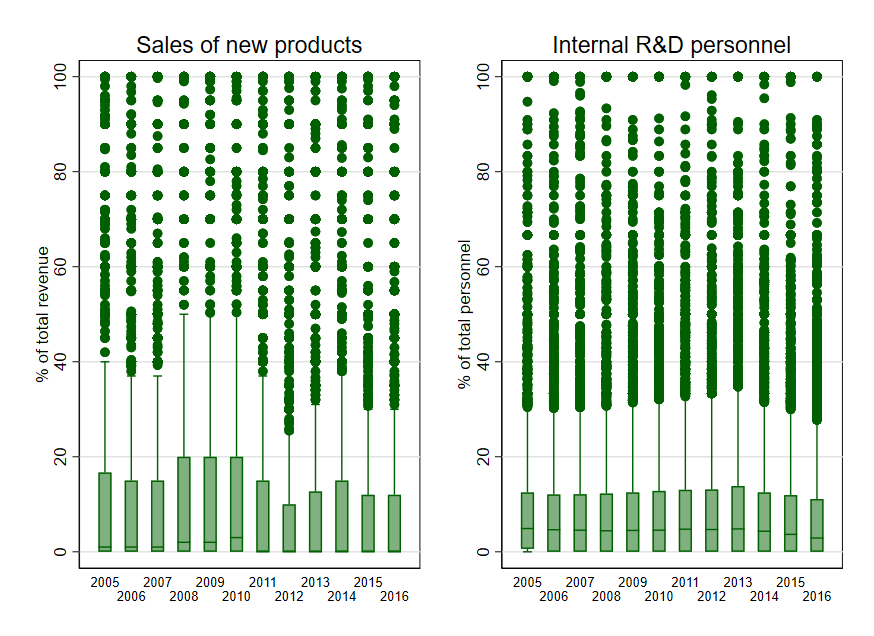
\includegraphics[width=1.0 \textwidth]{03_figures/combined}
  \label{fig:box}
\end{figure}
This is in accordance with the low degree of correlation shown in table \ref{tab:descriptive}. Furthermore, the bin scatterplot in figure \ref{fig:bin} does not show a convincing relation either.

\begin{figure}[H]
  \centering
  \caption{Scatter plot of internal R\&D personnel and sales of new products}
    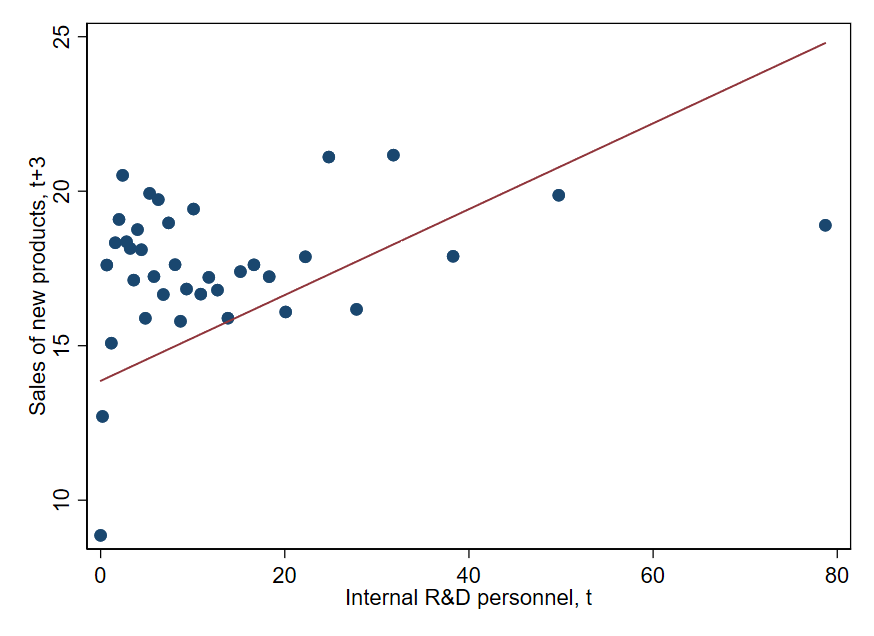
\includegraphics[width=1.0 \textwidth]{03_figures/scatter}
  \label{fig:bin}
\end{figure}
